\documentclass{standalone}

% Drawing
\usepackage{tikz}
\usepackage{pgfplots}
\pgfplotsset{compat=1.18}

% Define Color
\definecolor{safetyorange(blazeorange)}{rgb}{1.0, 0.4, 0.0}
\definecolor{royalblue(web)}{rgb}{0.25, 0.41, 0.88}

\begin{document}
	
	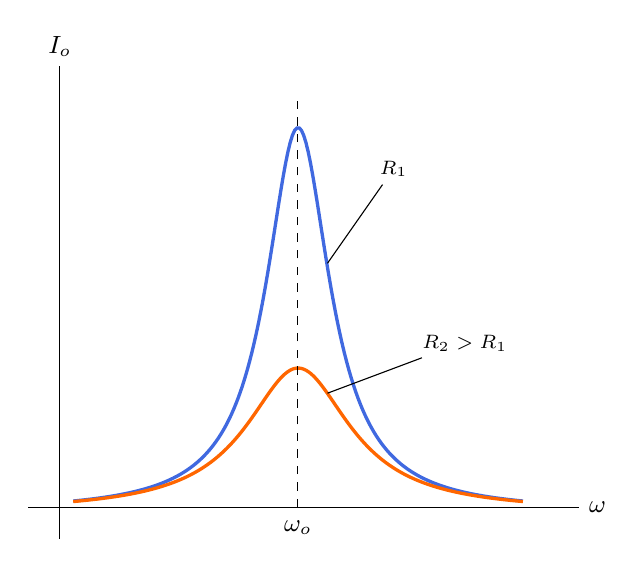
\begin{tikzpicture}
		% Grid
%		\draw[help lines] (0,0) grid (10,10);
		
		% Axis
		\draw (0,0.4) -- ++(7,0) node [right] {\small$\omega$};
		\draw (0.4,0) -- ++(0,6) node [above] {\small$I_o$};
		
		% Plot Function
		\begin{axis}[
			xtick=\empty,
			ytick=\empty,
			axis line style={draw=none},
			]
			%
			\addplot[royalblue(web), samples=200, very thick] {10/(3+ (2*x - 1/(1000*x))^2)};
			\addplot[safetyorange(blazeorange), samples=200, very thick] {10/(8+ (2*x - 1/(1000*x))^2)};
		\end{axis}
		
		% Text Labels
		%% x-Axis
		\draw [dashed] (3.424,0.4) -- ++(0,5.2) node [pos=-0.05] {\small$\omega_o$};
		%% On Plot
		\draw (4.5,4.5) -- (3.8,3.5) node [pos=-0.2] {\scriptsize$R_1$};
		\draw (5,2.3) -- (3.8,1.85) node [pos=0.1, above right] {\scriptsize$R_2>R_1$};
	\end{tikzpicture}
	
\end{document}